\begin{figure}[H]
    \centering
    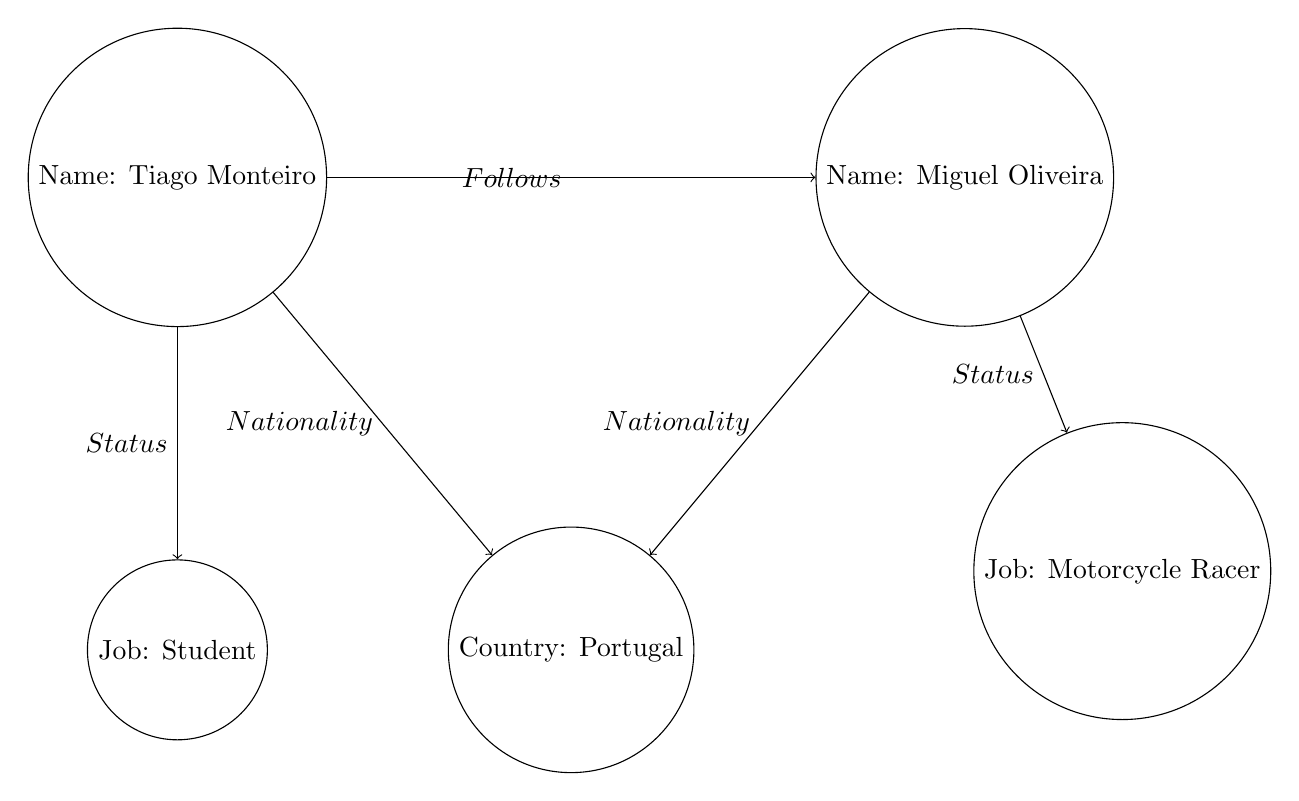
\begin{tikzpicture}
    \node[shape=circle,draw=black] (A) at (-5,3) {Name: Tiago Monteiro};
    \node[shape=circle,draw=black] (B) at (-5,-3) {Job: Student};
    \node[shape=circle,draw=black] (C) at (-0,-3) {Country: Portugal};
    \node[shape=circle,draw=black] (D) at (5,3) {Name: Miguel Oliveira
};
    \node[shape=circle,draw=black] (E) at (7,-2) {Job: Motorcycle Racer};

    

    \path [->](A) edge node[left] {$Status$} (B);
    \path [->](A) edge node[left] {$Nationality$} (C);
    \path [->](A) edge node[left] {$Follows$} (D);
    \path [->](D) edge node[left] {$Status$} (E);
    \path [->](D) edge node[left] {$Nationality$} (C);


    \end{tikzpicture}    
    \caption{Example of a simple social network in a graph data model.}
    \label{fig:graphmodel}
\end{figure}